%% LaTeX2e class for student theses
%% thesis.tex
%% 
%% Karlsruhe Institute of Technology
%% Institute for Program Structures and Data Organization
%% Chair for Software Design and Quality (SDQ)
%%
%% Dr.-Ing. Erik Burger
%% burger@kit.edu
%%
%% Version 1.3, 2016-12-29

%% Available languages: english,ngerman
%% Available modes: draft,final (see README)
\documentclass[ngerman,final]{sdqthesis}

%% ---------------------------------
%% | Information about the thesis  |
%% ---------------------------------

%% Name of the author
\author{Gruppe Nostrum\\Manuel Karl, Dominik Kleiser, Marc Leinweber, Nico Mürdter}

%% Title (and possibly subtitle) of the thesis
\title{Konzeption und Entwicklung einer parallelen Ray- \& Pathtracing-Anwendung}

%% Type of the thesis 
\thesistype{Projektpraktikum}

%% Change the institute here, ``IPD'' is default
% \myinstitute{Institute for \dots}

%% You can put a logo in the ``logos'' directory and include it here
%% instead of the SDQ logo
% \grouplogo{myfile}
%% Alternatively, you can disable the group logo
\nogrouplogo

%% The reviewers are the professors that grade your thesis
\reviewerone{Philip Pfaffe, Martin Tillmann}
\reviewertwo{Prof. B}

%% The advisors are PhDs or Postdocs
\advisorone{M.Sc. C}
%% The second advisor can be omitted
\advisortwo{M.Sc. D}

%% Please enter the start end end time of your thesis
\editingtime{28. November 2016}{05. Februar 2017}

\settitle

%% --------------------------------
%% | Settings for word separation |
%% --------------------------------

%% Describe separation hints here.
%% For more details, see 
%% http://en.wikibooks.org/wiki/LaTeX/Text_Formatting#Hyphenation
\hyphenation{
% me-ta-mo-del
Pro-gram-mie-rung
Punkt-licht-quel-len
}

%% --------------------------------
%% | Bibliography                 |
%% --------------------------------

%% Use biber instead of BibTeX, see README
\usepackage[citestyle=numeric,style=numeric,backend=biber]{biblatex}
\addbibresource{thesis.bib}

%% ====================================
%% ====================================
%% ||                                ||
%% || Beginning of the main document ||
%% ||                                ||
%% ====================================
%% ====================================
\begin{document}

%% Set PDF metadata
\setpdf

%% Set the title
\maketitle

%% The Preamble begins here
\frontmatter

\setcounter{page}{1}
\pagenumbering{roman}

%% ----------------
%% |   Abstract   |
%% ----------------
 
%% For theses written in English, an abstract both in English
%% and German is mandatory.
%%
%% For theses written in German, a German abstract is sufficient.
%%
%% The text is included from the following files:
%% - sections/abstract

%% ------------------------
%% |   Table of Contents  |
%% ------------------------

%% -----------------
%% |   Main part   |
%% -----------------

\mainmatter

\renewcommand{\cleardoublepage}{}
\renewcommand{\clearpage}{}
\setlength{\parindent}{0em} 

% -*- coding: iso-8859-1 -*-
% !TeX spellcheck = de_DE
% !TeX encoding = iso-8859-1

\chapter{Einleitung}
\label{ch:einleitung}

Ray- und Pathtracing sind Techniken mit hoher Bedeutung. Durch Computer erzeugte Grafiken, die nicht in Echtzeit berechnet werden, werden mit Hilfe von Ray- und Pathtracing-Technologien gerendert. Die Algorithmen verfolgen dabei Lichtstrahlen, um zu berechnen, ob ein Primitiv, das heißt ein Objekt der Szenerie, beleuchtet und nicht verdeckt ist.

Diese Arbeit entstand im Rahmen der Veranstaltung \glqq Praxis der Multikern-Programmie\-rung: Werkzeuge, Modelle, Sprachen\grqq \ der Fakultät für Informatik am Karlsruher Institut für Technologie. Ziel ist es, zunächst einen hochparallelen und effizienten Raytracer zu implementieren. In einem zweiten Teil wurde ein Pathtracer implementiert.

Beim Raytracing werden für jeden Pixel des zu rendernden Bildes zu allen Punktlichtquellen der Szene ein Strahl versendet. Trifft der Strahl die Lichtquelle und wird er nicht durch ein anderes Primitiv blockiert, wird der Punkt beleuchtet. Im hier implementierten Modell wurde ein Whitted-Style-Raytracer\footnote{\url{https://de.wikipedia.org/wiki/Raytracing}} ohne Reflektion mit Lambert-Schattierung implementiert. Hierbei handelt es sich um eine sehr einfache Variante, da Parallelisierung und Effizienz im Vordergrund standen.

Das Pathtracing ist eine stochastische Variante des Raytracings, die mit Hilfe von Monte-Carlo-Integration die globale Beleuchtung einer Bildstelle simuliert. Es werden statt Punktlichtquellen Flächenlichtquellen benutzt. Das bedeutet, dass die Primitive der Szene Licht emittieren können. Für jeden Strahl, der ein Szenerieobjekt trifft, werden $n$ zufällige Strahlen versendet, die wiederum bei einem Treffer neue Kindstrahlen erzeugen (\textit{Diffuses Raytracing}). Die Beleuchtung der Stelle ergibt sich aus der Beteiligung all dieser Strahlen.

In Kapitel \ref{ch:analyse} werden zunächst die Problemstellungen diskutiert und Ansätze zur Parallelisierung erörtert. Im anschließenden Kaptitel \ref{ch:implementierung} wird die Umsetzung der Ansätze beschrieben. Die Ergebnisse werden in Kapitel \ref{ch:evaluation} evaluiert. Mit Kapitel 5 wird diese Arbeit abgeschlossen.
% -*- coding: iso-8859-1 -*-
% !TeX spellcheck = de_DE
% !TeX encoding = iso-8859-1

\newpage
\chapter{Analyse und Entwurf}
\label{ch:analyse}
Das folgende Kapitel beschreibt die Analyse der Problemstellung und die betrachteten Ansätze zur Parallelisierung. Zu Beginn wurde eine naive und nicht parallelisierte Implementierung erstellt. Es wurde schnell klar, dass die reine Parallelisierung naiver Algorithmen nicht zielführend sind. So lag das Augenmerk bei der Suche nach effizienten und schnellen Algorithmen für Ray- bzw. Pathtracing. Des Weiteren war eine schnelle Datenstruktur von Nöten, um eine effiziente Traversierung der Primitive (Dreiecke) zu ermöglichen.

\section{Analyse der Problemstellung}
\subsection{Raytracing}
\label{sec:ray_tracer}
Der erste Raytracing-Ansatz bestand aus dem naiven Versuch, jeden Pixel Strahl zu verfolgen und eine einfache Schattenstrahlberechnung anzustellen. Dieser Ansatz lässt sich trivial parallelisieren. So konnte der naive Algorithmus mit OpenMP über alle Pixel paralellisiert werden. Hierbei wurde Datenparallelität benutzt. Als ein weiterführender Schritt wurde die Benutzung von Strahlenbündel eingeführt, welche mit Hilfe von Intel SSE-Instruktionen\footnote{\url{https://software.intel.com/sites/landingpage/IntrinsicsGuide}} realisiert wurden. Da eine der beiden Testmaschinen auch die verbesserte Version AVX unterstützt, wurde noch eine dritte Implementierung in AVX hinzugefügt.

Das Konzept der Strahlenbündel basiert auf der Annahme, dass die benachbarten Strahlen eines betrachteten Strahls mit hoher Wahrscheinlichkeit das gleiche Dreieck treffen und so auch die gleiche Traversierung der Datenstruktur vollziehen. Es lassen sich Bündel von Strahlen zusammenfassen und mit Hilfe von SSE-Instruktionen gleichzeitig betrachten. Da es sich bei SSE um interne Vektorinstruktionen handelt, welche pro Prozessorfaden getrennt voneinander operieren, ließ sich die Technik mit OpenMP kombinieren.

\subsection{Pathtracing}
\label{sec:path_tracer}
Anders als beim Rayrtracing kann man beim Pathtracing nicht auf Strahlenbündel setzen, da die \glqq Verfolgung\grqq\ eines Pfades auf zufälligen Richtungsänderungen basiert. Nur die von der Kamera wegführenden Strahlen besitzen die Eigenschaft, mit hoher Wahrscheinlichkeit das gleiche Dreieck zu treffen. Um dennoch eine gute Performanz beim Pathtracing zu erreichen, wurde hier auf die hochparallelisierte GPU gesetzt. Die Umsetzung ist hierbei ebenfalls ein datenparaller Ansatz über alle Pixel. Jeder GPU-Faden traversiert einen Pfad bis dieser terminiert.

\section{Datenstruktur}
\subsection{Räumliche Datenstruktur}
\label{sec:kdTree}
Die Suche nach geschnittenen Dreiecken ist einer der aufwendigsten Schritte bei Ray- bzw. Pathtracing. Der naive Ansatz war eine vollständige Suche auf allen Dreiecken. Dabei wurden die Dreiecke unabhängig ihrer räumlichen Position betrachtet. Diese Vorgehensweise ist sehr ineffizient und skaliert nicht. Eine effiziente Lösung bietet hierfür eine Bounding Volume Hirachy in Form eines k-d-Baums.

Die Dreiecke werden anhand ihrer räumlichen Position in Bereiche unterteilt. Dazu wird der Raum rekursiv entlang einer Achsendimension in zwei kleinere Teilbereiche unterteilt, bis jeder Bereich nur noch eine kleine Anzahl an Dreiecken enthält. Die Unterteilungsmetrik kann verschieden gewählt werden.
In einem ersten Ansatz wurde die naive Variante gewählt, bei der die Bereiche anhand des räumlichen Medians entlang der Achsendimension der größten Ausdehnung aufgeteilt wurden. Hierbei erhält man einen gut balancierten k-d-Baum.

Der zweite Ansatz bestand darin den k-d-Baum mit Hilfe der so genannten Surface Area Heuristic (SAH) zu teilen. Dabei werden die Kosten einer Bereichstraversierung gegenüber den Kosten für die Traversierung aller beinhalteten Dreicke abgeschätzt. Um hierbei ein gutes Minimum zu finden, werden alle Trennebenen miteinander verglichen. Die Trennebene mit den geringsten zukünftigen Bereichskosten gewinnt. Kann keine Trennebene gefunden werden, sodass die Traversierungskosten für alle Dreiecken größer als die einer Aufteilung sind, bricht die Rekursion ab.

Damit bei den beschriebenen Abläufen der Kopieraufwand für die Dreicke die Laufzeit nicht beeinträchtigt, wurden die Dreicke nur über ihren Index im ursprünglichen Vektor identifiziert. Dieses Konzept der Indirektion über Verktorindizes zieht sich durch sämtliche Teile des Projekts.

\subsection{Axis Aligned Bounding Boxes und Dreiecksschnitt}
%\subsection{Axis Aligned Bounding Boxes}
Die Bereiche mit denen im oben beschriebenen k-d-Baum die Dreiecke räumlich unterteilt werden, können verschieden realisiert werden. Da in der hier verwendeten Implementierung nur an Achsen getrennt wird, sind die Bereiche an den Achsendimensionen orientiert. Man spricht von Axis Aligned Bounding Boxes. Hieraus ergeben sich noch weitere Vorteile. So kann man die ganze Bounding Box (im folgenden \glqq BB\grqq) allein durch zwei Punkte darstellen, welche die minimale bzw. maximale Ausdehnung der Box darstellen. Des Weiteren werden Schnitte einfacher, da man sich an den Achsendimensionen orientieren kann.

%\subsection{Dreiecke und Dreiecksschnitt}
Die Dreiecksschnittberechnung ist eine der am meisten verwendeten Funktionen im gesamten Projekt. Deshalb wirkt sich ein effizienter Algorithmus hier sehr stark auf die Gesamtlaufzeit aus. Um dies zu realisieren, wurde der Dreiecksschnittalgorithmus von Tomas Möller und Ben Trumbore verwendet \cite{moller2005fast}.  

\section{Parallelisierungsansätze}
\subsection{OpenMP}
\label{sec:openmp}
Aufgrund der oben beschriebenen Datenparallelität beim Raytracing, bietet sich eine Parallelisierung mittels OpenMP an. Hier können Schleifen durch Direktiven an den Übersetzer parallelisiert werden: \code{\#pragma omp parallel for}. Die Schleife wird in gleich große Abschnitte unterteilt, die jeweils von einem Thread abgearbeitet werden. Dies ist besonders nützlich bei der Schnittberechnung, die für jeden Pixel durchgeführt werden muss. Zu beachten ist, dass die einzelnen Schleifeniterationen keine Abhängigkeiten voneinander haben dürfen.
Durch die rekursive Erzeugung des k-d-Baums ergibt sich die Möglichkeit des Taskparallismus mittels \code{\#pragma omp task}.
Somit kann ein Thread \glqq Arbeitspakete\grqq\ erstellen, die von weiteren Fäden bearbeitet werden. Hierbei ist eine Begrenzung der Task-Tiefe wichtig, da ab einer gewissen Tiefe der Mehraufwand zwischen Task-Erzeugung und Task-Bearbeitung zu groß wird und ein Verlust an Effizienz eintritt.

OpenMP bietet sich im speziellen an, da die von OpenMP verwendeten Direktiven immer lauffähig sind und mittels einfacher Compiler-Flags aktiviert werden können. Es ist somit möglich einfach inkrementell zu parallelisieren. 

\subsection{Strahlschnittparallelisierung mit SIMD-Anweisungen}
\label{sec:sse}
Durch die explizite Vektorisierung der Strahlen können mehrere Schnittberechnungen gleichzeitig durchgeführt werden. Dies wird erreicht, indem die Strahlen, repräsentiert durch mehrere 32 Bit Gleitkommazahlen, abhängig vom Prozessor durch AVX- bzw. SSE-Instruktionen bearbeitet werden. Bei AVX Instruktionen können 256 Bit große Register, bei SSE Instruktionen 128 Bit große Register benutzt werden. So ist es es möglich vier (SSE) oder acht (AVX) Strahlen in einem Register zu speichern. Anschließend können die Schnittberechnungen auf das Register angewandt werden. 
%Da wie bereits AVX- und SSE-Instruktionen mit weiteren Parallelisierungsmöglichkeiten zusammen funktionieren können bei einem Prozessor mit 4 Kernen und AVX bis zu 32 Strahlen gleichzeitig berechnet werden.

\subsection{Massive SIMD-Parallelisierung auf der GPU}
\todo{CUDA-Impl für PT erklären}
Aufgrund der exponentiell steigenden Anzahl an Strahlen beim Pathtracing, bietet sich hier die Parallelisierung auf der GPU an. Diese bietet eine sehr hohe Anzahl an Fäden, sodass jeder Strahl von einem Faden bearbeitet werden kann. Abzuwägen ist hierbei der Mehraufwand zwischen Kopieraufwand von CPU auf GPU im Vergleich zur hoch parallelen Datenverarbeitung auf der GPU. 

Ein Problem der GPU stellt die rekursive Berechnung der Schnitttests und der Datenstruktur dar. Die GPU ist nicht für rekursive Funktionalitäten ausgelegt. Des Weiteren sollte man aufgrund des Locksteps innerhalb eines GPU-Warps möglichst auf Kontrollstrukturen verzichten. Bei einer bedingten Verzweigung müssen beide möglichen Wege von allen 32 Fäden durchlaufen werden. Nicht verwendbare Ergebnisse werden anschließend verworfen. Man erzeugt somit im schlimmsten Fall den doppelten Rechenaufwand pro Warp. 
% -*- coding: iso-8859-1 -*-
% !TeX spellcheck = de_DE
% !TeX encoding = iso-8859-1

\chapter{Umsetzung und Implementierung}
\label{ch:implementierung}

Zur Umsetzung des Projekts wurde uns von Seiten des Lehrstuhls ein GitLab-Repository mit integriertem Continuous-Integration-Server (CI-Server) zur Verfügung gestellt. Programmiert wurde in portablem und modernem C++ (im aktuellen Standard \textit{C++14}).  Außerdem haben wir uns für das Buildsystem \textit{cmake} und für die graphische Entwicklungsumgebung \textit{CLion} entschieden. Die meiste Zeit wurde via \textit{Teamviewer} mit der aus der agilen Softwareentwicklung bekannten Arbeitstechnik \textit{Paarprogrammierung} gearbeitet.

Ziel war es, kompatible Software für zwei vorgegebene Test- und Benchmark-Systeme zu entwickeln (im Folgenden \textit{i41pc189} und \textit{i41pc205} genannt). Die Anwendung wurde aber für alle gängigen Systeme ausgelegt; Programmcode und CMake-Konfiguration wurden so eingerichtet, dass nur für die aktuelle Umgebung kompatible Maschinenbefehle kompiliert werden (z.B. Abschalten von AVX bei fehlender Hardwareunterstützung).

Die einzigen von der Aufgabenstellung zugelassenen Bibliotheken waren:
\begin{itemize}[noitemsep,topsep=0pt,parsep=0pt,partopsep=0pt]
\item \url{https://github.com/nothings/stb} zum Schreiben von Bitmaps,
\item \url{https://nlohmann.github.io/json/} zum Lesen von JSON-Dateien,
\item \url{https://github.com/syoyo/tinyobjload} zum Laden von OBJ-Dateien
\end{itemize}
sowie die NVIDIA Bibliotheken \textit{CUDA} und \textit{Thrust} zur Programmierung der Grafikkarte (GPGPU-Programmierung).

\section{Software-Architektur}
Beide Aufgabenteile (Raytracing und Pathtracing) mussten in einer gemeinsamen Anwendung implementiert werden. Welches der beiden Tracing-Verfahren zum Einsatz kommt wird dabei dynamisch zur Laufzeit aus der Szenen-Beschreibung (JSON-Datei) ausgelesen. Da anfangs noch mit Anpassungen und Erweiterungen der Aufgabenstellung zu rechnen war, entschieden wir uns für einen möglichst modularen und objektorientierten Software-Entwurf. Eine Auflistung und Beschreibung der entwickelten Module findet sich in \autoref{tbl:moduls}. 

Der Programmablauf ließ sich in die folgenden Schritte untergliedern:
\begin{enumerate}
\item Dateieingabe: Lesen der Szenen-Beschreibung (JSON) und Obj-Datei
\item Vorverarbeitung der Szene: Vorberechnungen für die Dreiecke (z.B. Berechnung der Normalen), Konstruieren des k-d-Baums und Berechnung der Primärstrahlen; in diesem Schritt werden auch anhand der Szene Weichen für das weitere Vorgehen gestellt (Wahl des k-d-Baums, Entscheidung, ob GPU verwendet werden soll)
\item Rendering: Durchführung des Tracing-Verfahrens
\item Dateiausgabe: Schreiben des Ergebnisbildes in eine Bitmap-Datei
\end{enumerate}

\begin {table}[htbp]
	\begin{center}
    \begin{tabular}{ | l | p{10cm} |}
    \hline
    \textbf{Modulname} & \textbf{Beschreibung} \\ \hline
    main.h & Einstiegspunkt mit Mainfunktion; verbindet die Komponenten miteinander und misst deren Ausführungszeiten. \\ \hline
    options.h & Datei zum Setzen verschiedenerer statischer Programmparameter; zum Ein- und Ausschalten von AVX, SSE und CUDA. \\ \hline
    io.h & Zuständig für das Parsen der JSON-Szenen-Beschreibung und der Wavefront OBJ-Datei.\\ \hline
    scene\_preprocessor.h & Vorverarbeitung der Szene (siehe oben). \\ \hline
    pray.h & Mit dem Aufruf von \texttt{render(...)} wird das Tracing-Verfahren gestartet; die Entscheidung ob Ray- oder Pathtracing durchgeführt wird, wird anhand der Informationen aus dem Szene-Objekt (Parameter) entschieden. \\ \hline
    geometry.h & Definiert die benötigten geometrischen Primitiven (\textit{Vec3}, \textit{Triangle}, \textit{Bounding Box}, usw.) und die auf ihnen ausgeführten Algorithmen (z.B. Dreieck- und BB-Schnitt). \\ \hline
    geometry\_simd.h & Erweitert die Algorithmen aus \textit{geometry.h} um deren SSE und AVX Pendants (Intrinsics). \\ \hline
    spatial.h  & \multirow{4}{*}{\parbox{10cm}{Schnittstelle für räumliche Datenstrukturen und die\newline dazugehörigen Instanziierungen (siehe \autoref{sec:spatial}).}} \\ 
    bf\_search.h & \\
    kd\_tree.h & \\ 
    kd\_tree\_sah.h & \\ 
    kd\_tree\_hybrid.h & \\ \hline
	path\_trace.cu.h & \multirow{4}{*}{\parbox{10cm}{CUDA-Code für paralleles Pathtracing auf der GPU.}} \\
    kd\_tree\_gpu.h & \\
    gpu\_util.h & \\ \hline
    \end{tabular}
    \caption {Beschreibung der Module}
    \label{tbl:moduls}
	\end{center}
\end {table}

\section{Implementierung der räumlichen Datenstruktur}\label{sec:spatial}
Es wurde schnell klar, dass die Schnittberechnung der Dreiecke mit den Strahlen der Flaschenhals der Laufzeit werden würde. Um hier möglichst einfach zwischen alternativen räumlichen Datenstrukturen wechseln zu können, entschieden wir uns für eine Vererbungshierarchie wie in \autoref{img:spatial} dargestellt.

\begin{figure}[htbp]
	\centering
	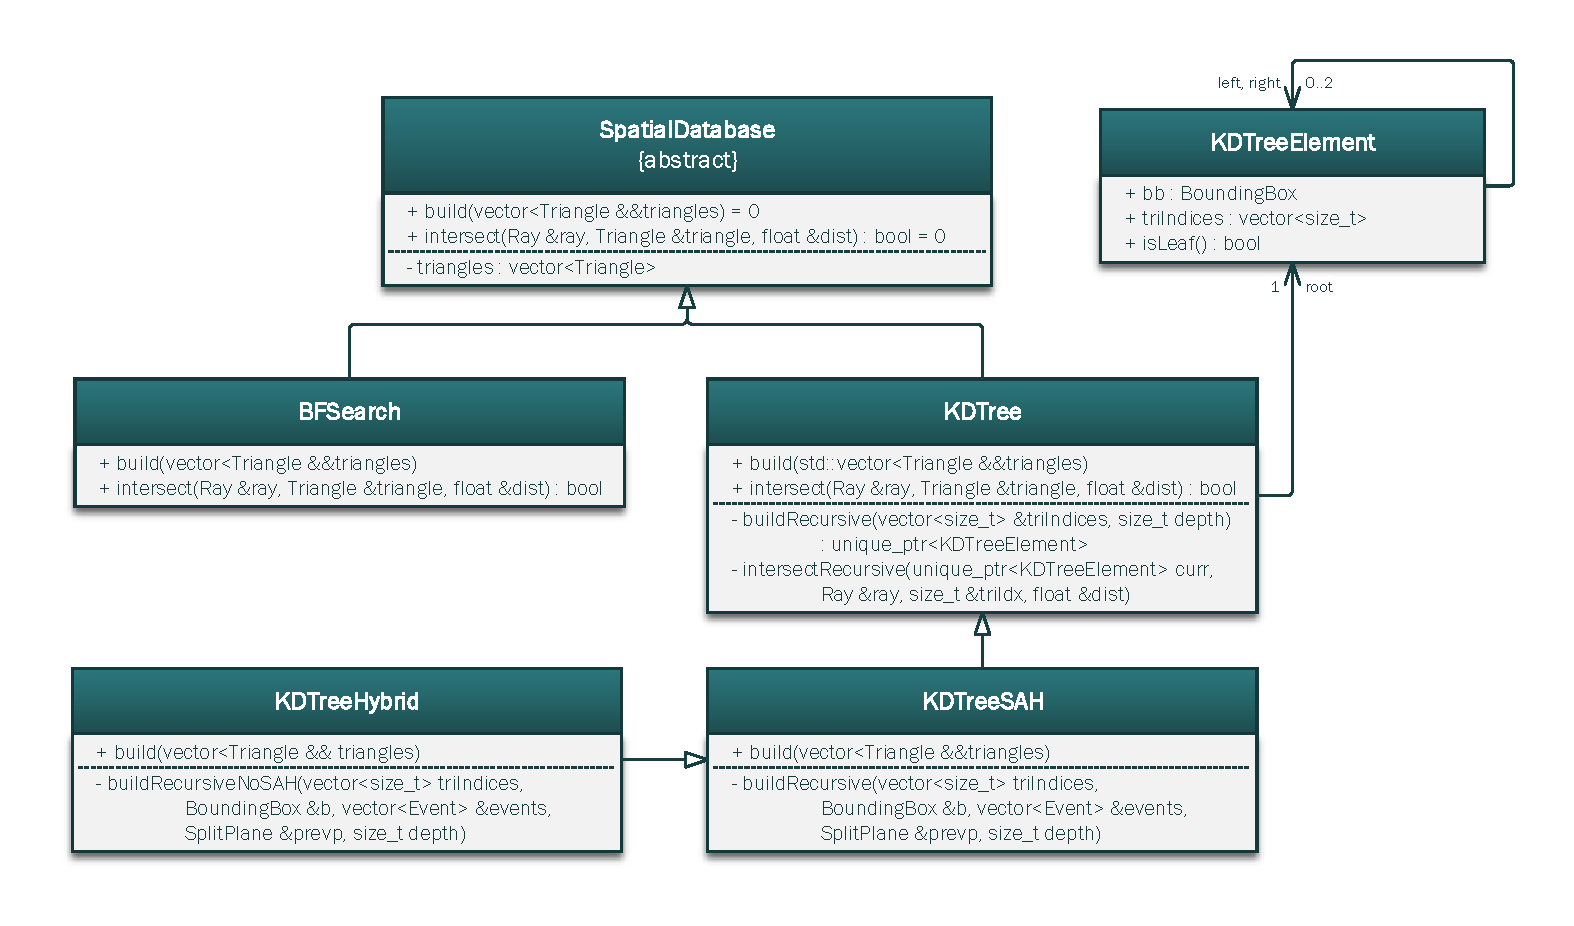
\includegraphics[width=1\textwidth]{graphics/spatial.pdf}
	\caption{Klassendiagramm: Räumliche Datenstruktur}
	\label{img:spatial}
\end{figure}

Die Klasse \texttt{SpatialDatabase} stellt zwei abstrakte Methoden \texttt{build} und \texttt{intersect} bereit. Diese werden dann von den Unterklassen \texttt{BFSearch} und \texttt{KDTree} implementiert. \texttt{BFSearch} führt bei der Schnittberechnung eine vollständige Suche über alle Dreiecke durch. Beim bauen wird lediglich ein \textit{move} aller Dreiecke in die Instanzvariable \textit{triangles} vorgenommen.
In \texttt{KDTree} wird in \texttt{build} ein naiver k-d-Baum aufgebaut. \texttt{KDTreeSAH} erzeugt k-d-Bäume gemäß der Surface-Area-Heuristik. Die Schnittberechnung von \texttt{KDTreeSAH} wird von  \texttt{KDTree} geerbt.

Der Aufbau der beiden k-d-Bäume erfolgt rekursiv und wurde wie in \autoref{sec:openmp} beschrieben mit \textit{OpenMP}-Tasks parallelisiert. Neue Tasks werden jedoch nur bis zu einer bestimmten Tiefe \textbf{TASK\_DEPTH} erzeugt. Die maximale Tiefe des konstruierten Baums und die Mindestzahl benötigter Dreiecke für einen weitere Teilung sind durch die beiden Parameter \textbf{MAX\_DEPTH} und \textbf{THRESHOLD} beschränkt.
Für die Konstruktion des Baums mit SAH wurde zunächst der Algorithmen in $\mathcal{O}(n\log^2{}n)$\ aus \cite{wald2006building} implementiert. Später wurde dann zur Beschleunigung ein Wechsel auf den $\mathcal{O}(n\log{}n)$-Algorithmus vorgenommen.

\section{Implementierung des Raytracers}
Der Raytracer wurde zunächst in einer möglichst einfachen, sequentiellen Variante entworfen. Der Dreiecksschnitt wurde von Anfang an mit dem Möller–Trumbore-Schnitt\-algorithmus durchgeführt. Im nächsten Schritt wurde die vollständige Suche nach dem Dreieck mit geringstem Abstand durch eine wesentliche effizientere Suche in einem k-d-Baum ersetzt (siehe \autoref{sec:kdTree} und \autoref{sec:spatial}). Der erste Ansatz zur Parallelisierung war eine Verteilung der Bildpixel/Primärstrahlen auf mehrere Threads. Da hierbei keine Abhängigkeiten zwischen Pixeln existieren (\textit{embarrassingly parallel}), konnte dies auf einfache Weise mit OpenMP vorgenommen werden.
Eine weitere Beschleunigung konnte anschließend durch die Bündelung von Strahlen erreicht werden (siehe \autoref{sec:ray_tracer}). Da die Testmaschine \textit{i41pc205} keine AVX-Instruktionen unterstützt, entschieden wir uns dafür, abhängig von der Zielplattform, unser Programm sowohl für SSE (vier Strahlen) als auch für AVX (acht Strahlen) zu optimieren. Da jeder Prozessor seine eigenen SIMD-Register besitzt, skaliert dieser Ansatz auch äußerst gut mit der vorherigen Parallelisierung mit \textit{OpenMP}. Um auf die hardwarenahen SIMD-Instruktionen zurückzugreifen, wurden intrinsische Funktionen (Intrinsics) verwendet. Hierzu musste der Möller-Trumbore-Algorithmus für SIMD umgeschrieben werden und es waren Anpassungen in der k-d-Baum Schnittberechnung erforderlich.

\section{Implementierung des Pathtracers}
Eine erste Version des Pathtracers konnte durch nur wenige Anpassungen am schon vorhandenen Raytracer implementiert werden. Es zeigte sich jedoch, dass aufgrund der mit der Rekursionstiefe exponentiell wachsenden Anzahl Strahlen eine reine Parallelisierung über die Pixel zu unzufriedenstellenden Laufzeiten führt.
Wie in \autoref{sec:path_tracer} beschrieben ist eine Parallelisierung des Pathtracings mit den SIMD-Registern der CPU nur eingeschränkt sinnvoll.
Um das Tracing auf der GPU durchführen zu können mussten viele der schon vorhandenen Funktionen aus \texttt{geometry.h} in CUDA-Kernel-Code überführt werden. Außerdem muss der k-d-Baum in eine für die GPU besser geeignete Form umkopiert werden. Bei der Implementierung des Verfahrens in CUDA kam es zu mehreren Schwierigkeiten: 
\begin{itemize}
\item Da das Programmiermodell von Grafikkarten nicht für rekursive Funktionsaufrufe ausgelegt ist, versuchten wir in unserem ersten Lösungsansatz diese aus dem Programmcode zu eliminieren. Dazu mussten in einem Array alle Strahlen (über alle Pixel) auf der momentanen Rekursionstiefe zwischengespeichert werden. Dieser Ansatz musste später aufgrund eines zu hohen Speicherverbrauches (sowohl auf der GPU als auch auf der CPU) verworfen werden.
\item Bei der rekursiven Variante kam es ebenfalls zu Problemen mit dem GPU-Speicher. Hier kommt es zu einer zweifachen Rekursion: Einerseits die beim Pathtracing vorgebenene Rekursion beim Auftreffen auf ein Dreieck, andererseits der rekursive Abstieg auf dem k-d-Baum für die Schnittberechnung. Eine \glqq Stackless\grqq-Traversierung (siehe \cite{popov2007stackless}) des k-d-Baum gestaltete sich als deutlich schwieriger zu implementieren als zunächst erwartet.
\item Eng verwandt mit dem vorherigen Punkt ist die Festellung, dass ein k-d-Baum der gemäß der SAH-Metrik aufgebaut wurde, nur eingeschränkt für die GPU geeignet ist. SAH neigt dazu deutlich tiefere Bäume zu erzeugen, was bei der Traversierung zu einer größeren Rekursionstiefe führt. Mit einem naiven k-d-Baum konnten teilweise deutlich bessere Laufzeiten erzielt werden. Um ein gutes Mittelmaß bei den Laufzeiten zu finden, wurde eine SAH-Abwandlung eingeführt, welche auf den ersten Ebenen die naive Unterteilungsmetrik verwendet und erst dann auf SAH wechselt. Siehe \texttt{KDTreeHybrid} in \ref{img:spatial}.
\end{itemize}

Da andere Gruppen beim Pathtracing deutlich geringere Laufzeiten erzielten als unsererer Meinung nach mit dem vorgeschriebenem Algorithmus (auch als \textit{diffuses Raytracing} bezeichnet) möglich ist, wurde ebenfalls noch eine etwas abgewandelte Variante des Verfahrens implementiert. Bei dem in \autocite{Kajiya:1986:RE:15886.15902} vorgestellten Algorithmus zum Pathtracing wird nicht bei jedem Treffer auf ein Objekt ein neuer Strahl erzeugt, stattdessen wird \textbf{NUM\_SAMPLES} oft über jedes der Pixel iteriert und jeweils nur ein Pfad verfolgt. Am Ende wird der berechnete Pixelwert dann durch \textbf{NUM\_SAMPLES} geteilt. Dies führt zu vergleichbaren Ergebnisbildern, erzeugt aber bei Rekursionstiefen größer eins deutlich weniger Strahlen; die Anzahl der Strahlen ist linear und nicht exponentiell zu \textbf{NUM\_SAMPLES}.





\chapter{Evaluation}
\label{ch:evaluation}
In diesem Kapitel wird die Leisungsfähigkeit der Implementierung mit Hilfe verschiedener Benchmarks und Vergleiche untersucht.

\begin{table}[h]
	\centering
	\caption{Eigenschaften der Szenen}
	\label{tbl:local_scenes}
	\begin{tabular}{|c|c|c|c|c|c|}
		\hline
		Szene 			& Auflösung & Dreiecke	& Lichtquellen & Rekursiontiefe & Samples \\ \hline
		Cube  			& 8000x6000 & 12 	& 2	& -	& -			\\
		Sponza  		& 2048x2048 & 262267 	& 1 & -	& -			\\
        Cornell (PT) 	& 800x600 & 14 	& 8			& 1	& 4000	\\
		Sponza (PT) 	& 400x400 & 262267 & 12			& 1	& 32	\\
		\hline
	\end{tabular}
\end{table}

\begin{table}[h]
	\centering
	\caption{Laufzeiten der lokalen Benchmarks}
	\label{tbl:local_bench}
	\begin{tabular}{|c|c|c|c|c|c|c|}
		\hline
		Szene 			& naiv		& k-d-Baum	& + AVX		& + SAH		& GPU 		& Heuristik \\ \hline
		Cube  			& 00:03:84 	& 00:03:73  & 00:03:42	& 00:03:21	& -			& 00:03:50	\\
		Sponza  		& $\infty$ 	& 01:41:17 	& 00:21:51  & 00:06:79	& -			& 00:06:38	\\
		Cornell (PT) 	& $\infty$ 	& 01:22:01 	& -			& 01:25:76	& 00:22:31	& 00:20:05	\\
		Sponza (PT) 	& $\infty$ 	& 07:17:73	& -			& 00:17:84	& 01:29:12	& 00:17:71	\\
		\hline
	\end{tabular}
\end{table}

\section{Hauptspeicher}
Für eine Szene mit 262267 Primitiven wird während des kompletten Renderprozesses ungefähr 1GB Hauptspeicher benutzt. Soll die Szene auf der GPU berechnet werden, wird geprüft, ob die zu benutzende GPU über genug Speicher verfügt. 

\section{Laufzeit}
Die Implementierung wurde auf den Praktikumssystemen sowie auf einer Enticklungsmaschine (im Folgenden \glqq lokaler Benchmark\grqq) in der Laufzeit evaluiert. Die lokalen Benchmarks wurden auf einem System mit Ubuntu 16.04, Intel Core i5-6600K CPU @ 3.50GHz, 32 GB Hauptspeicher und einer Nvidia Geforce GTX 1070 Grafikkarte mit 8 GB Grafikspeicher ausgeführt.  In Tabelle \ref{tbl:local_bench} sind die Zeiten des lokalen Benchmarks aufgelistet. Getestet wurden vier verschiedene Szenen (Cube, Sponza, Cornell-Box mit Pathtracing und Sponza mit Pathtracing). In Tabelle \ref{tbl:local_scenes} sind die Eigenschaften der Benchmarkszenen gelistet. Bei Pathtracing handelt es sich um Flächenlichtquellen. Das heißt es gibt Flächen die Licht emittieren und keine gesonderten Punktlichtquellen. Verglichen werden naive Implementierung (vollständige Suche), k-d-Baum, k-d-Baum mit AVX-Strahlbündelschnitt, selbiger mit SAH-Heuristik und für die Pathtracing-Szenen das Rendern auf der GPU (Nutzung des trivialen k-d-Baumes). Die Spalte Heuristik zeigt die erreichten Zeiten, wenn die Implementierung Datenstruktur und Ausführungsumgebung selbst wählt. Alle Benchmarkes wurden OpenMP-parallelisiert ausgeführt.

Nachfolgend sind die Ergebnisse der Benchmarks der Wettbewerbsmaschinen zu sehen. In Abbildung \ref{img:ptnormal} sind die Ergebnisse mit dem Pathtracing Algorithmus aus \cite{Kajiya:1986:RE:15886.15902} zu sehen und in \ref{img:ptdiffuse} sind die Ergebnisse mit dem vorgegebenen Algorithmus zu sehen.

\begin{figure}[htbp]
	\centering
	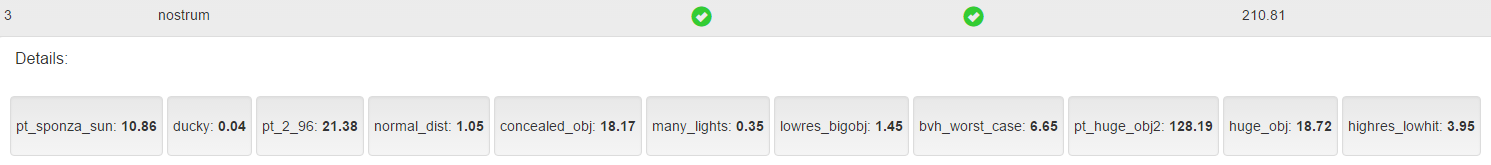
\includegraphics[width=1\textwidth]{graphics/nostrum_benches_avx_nogpu_ptnormal.PNG}
	\caption{Wettbewerbsmaschine \textit{i41pc189}: Pathtrace Algorithmus aus \cite{Kajiya:1986:RE:15886.15902}}
	\label{img:ptnormal}
\end{figure}

\begin{figure}[htbp]
	\centering
	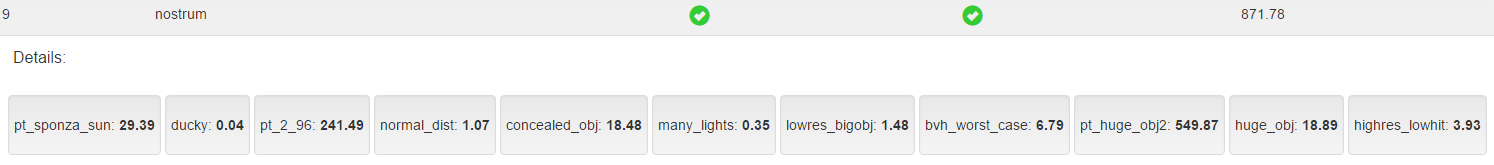
\includegraphics[width=1\textwidth]{graphics/nostrum_benches_avx_nogpu_ptdiffuse.PNG}
	\caption{Wettbewerbsmaschine \textit{i41pc189}: Vorgegebener Pathtrace Algorithmus}
	\label{img:ptdiffuse}
\end{figure}

\newpage
\chapter{Fazit}
\label{ch:fazit}

In dieser Arbeit wurde ein massiv paralleler Raytracer sowie ein Pathtracer implementiert. Dazu wurden die Problemstellungen analysiert und vorhandene Arbeiten auf ihre Tauglichkeit untersucht. Aufgrund dieser Ergebnisse wurde ein CPU-Raytracer mit zwei verschiedenen Datenstrukturen (k-d-Baum mit und ohne SAH-Heuristik) sowie ein CPU- und GPU-Pathtracer implementiert. 

Während der Arbeit zeigte sich, dass Wahl und Aufbau der Datenstruktur stark am Erfolg einer effizienten Lösung teilhaben. Trotz der zunächst trivial erscheinenden Parallelisierung, ergaben sich Probleme gerade für sehr große Szenen. Neben der Datenstruktur war auch das Pathtracing aufgrund des exponentiellen Wachstums schwer zu bewältigen. Es ergaben sich große Probleme bei der Wahl der Ausführungsumgebung (GPU vs CPU). Nichtsdestotrotz konnten auch für sehr große Szenen sehr gute Renderzeiten bei Full-HD-Auflösungen erreicht werden.

Als offene Punkte bleiben die stapelfreie Implementierung des GPGPU-Pathtracing und des k-d-Baum-Schnittes sowie eine Evaluierung des Raytracings auf der GPU.



%% --------------------
%% |   Bibliography   |
%% --------------------

%% Add entry to the table of contents for the bibliography
\nocite{*}
\printbibliography[heading=bibintoc]

\end{document}
